\section{Probing}
\label{sec:probing}

Probing methods aim to determine whether a given semantic concept is encoded within the \gls{ls} of a \gls{nn} \cite{li2024emergentworldrepresentationsexploring, karvonen2024emergentworldmodelslatent}.
The idea behind these methods is that if a concept can be reliably decoded from \gls{lr}, it is likely relevant to the problem being solved.
Studying such concepts can therefore provide insight into how the network internally represents the problem.

A probing analysis begins by identifying a set of semantic concepts that the network could potentially use to accomplish its task.
Each example in the dataset is then annotated to indicate the presence or absence of the studied concepts.
We denote by $c_j$ the presence or absence of concept $j$ in example $x$.
The dataset can therefore be written as follows:
\[
\mathcal{D} = \{(x^{(i)}, y^{(i)}, c^{(i)}_1, \dots, c^{(i)}_n)\}_{i=1}^{N}.
\]

The data are subsequently projected into the \gls{ls} of the pretrained model.
For an input $x$, we write $\latentRepresentation[l](x) \in \mathbb{R}^{n_l}$, or simply $\latentRepresentation[l]$, the \gls{lr} obtained at layer $l$.
A classifier, referred to as a probe, is then trained to predict the presence of a given concept from this \gls{lr}.
It is denoted by $p_{\theta}^{l,j}$, where $\theta$ represents its parameters, $l$ indicates the layer from which the \gls{lr} is extracted, and $j$ identifies the concept being predicted.
The probe maps the \gls{lr} to a scalar value in $[0,1]$, which can be interpreted as the probability that the concept is present.
The parameters $\theta$ are learned by minimizing a loss function over the training examples using \gls{sgd}.
This gives the following mathematical formulation:
\begin{equation}
p_{\theta}^{l,j} : \mathbb{R}^{n_l} \rightarrow [0,1],
\qquad
\min_{\theta} \frac{1}{N} \sum_{i=1}^{N}
\mathcal{L}\left(
p_{\theta}^{l,j}\left(\latentRepresentation[l](x^{(i)})\right),
c_j^{(i)}
\right).
\label{eq:probe_function}
\end{equation}

The architecture of the probe must be kept intentionally simple.
A probe with excessive expressive capacity may be able to predict the concept by exploiting complex patterns within the representation.
These patterns do not necessarily indicate that the concept is explicitly encoded in the \gls{ls}.
Instead, they may result from the ability of the probe itself to combine and transform the available information.
Consequently, a highly expressive probe makes it difficult to distinguish between information that is directly accessible in the representation and information that is reconstructed by the classifier.
Restricting the capacity of the probe therefore helps ensure that its predictions primarily reflect the information already present in the \gls{ls}.

For this reason, probing methods often rely on linear classifiers.
A linear separation suggests that the information is easily accessible to the \gls{nn} and potentially usable during decision-making.
If the classifier achieves performance significantly above chance level, this suggests that the \gls{ls} contains exploitable information related to the considered concept.

Figure~\ref{fig:probes_decision_boundaries} illustrates the decision boundaries of such linear probes for three concepts, where each colored region indicates the area classified positively by the corresponding probe.

\begin{figure}[t]
\centering

% ================================================================
%  latent_space_shared.tex
%  Couleurs, macros et styles partagés par toutes les figures
%  latent_space_*.tex
%  Usage : % ================================================================
%  latent_space_shared.tex
%  Couleurs, macros et styles partagés par toutes les figures
%  latent_space_*.tex
%  Usage : \input{figures/latent_space/latent_space_shared.tex}
% ================================================================

% ----------------------------------------------------------------
% Couleurs des clusters
% ----------------------------------------------------------------
\colorlet{colorA}{blue!70!cyan}
\colorlet{colorB}{orange}
\colorlet{colorC}{green!60!black}

% Couleurs de directions (latent_space_directions.tex)
\colorlet{colorDirBA}{violet}
\colorlet{colorDirBC}{red!70!black}

% ----------------------------------------------------------------
% Macros de dessin
% ----------------------------------------------------------------
\input{figures/latent_space/plot_points.tex}
\input{figures/latent_space/plot_ellipse.tex}
\input{figures/latent_space/plot_probe.tex}
\input{figures/latent_space/plot_direction.tex}

% ----------------------------------------------------------------
% Styles d'axe partagés
% ----------------------------------------------------------------
\pgfplotsset{
  % Axe standard (clustering, probing, directions)
  latent axis/.style={
    width=11cm,
    height=10cm,
    xmin=-7, xmax=8,
    ymin=-7, ymax=5.5,
    axis x line=bottom,
    axis y line=left,
    axis line style={
      -{Stealth[length=8pt, width=6pt]},
      thick
    },
    ticks=none,
    xlabel={},
    ylabel={},
    clip=true,
  },
  % Variante panneau carré (latent_space_sparse_autoencoders.tex)
  latent panel/.style={
    latent axis,
    width=9cm,
    height=9cm,
  },
  % Variante petit panneau (latent_space_embeddings.tex)
  % N.B. width/height sont passés explicitement par chaque fichier
  % via width=\lsePanelWd, height=\lsePanelHt dans l'axe.
  latent embed/.style={
    latent axis,
    every axis plot/.append style={forget plot},
  },
}

% ================================================================

% ----------------------------------------------------------------
% Couleurs des clusters
% ----------------------------------------------------------------
\colorlet{colorA}{blue!70!cyan}
\colorlet{colorB}{orange}
\colorlet{colorC}{green!60!black}

% Couleurs de directions (latent_space_directions.tex)
\colorlet{colorDirBA}{violet}
\colorlet{colorDirBC}{red!70!black}

% ----------------------------------------------------------------
% Macros de dessin
% ----------------------------------------------------------------
% ================================================================
%  \plotPoints — Reusable macro to render a point cloud from file
%
%  Usage:
%    \plotPoints[color=<c>, size=<s>, opacity=<o>]{<file.data>}
%
%  Arguments (all optional, defaults shown below):
%    color   : fill & stroke color of the markers  (default: black)
%    size    : marker radius                        (default: 2pt)
%    opacity : fill opacity [0..1]                  (default: 0.85)
%
%  Positional (mandatory):
%    #1 : path to a whitespace-separated x y data file
%         (lines starting with % are treated as comments)
%
%  Example:
%    \plotPoints[color=blue!70!cyan, size=3pt]{data/cluster_a.data}
% ================================================================
\pgfkeys{
  /plotPoints/.is family, /plotPoints,
  % --- defaults ---
  color/.initial   = black,
  size/.initial    = 2pt,
  opacity/.initial = 0.85,
}

\newcommand{\plotPoints}[2][]{%
  \pgfkeys{/plotPoints, #1}%                     % apply user overrides
  \pgfkeysgetvalue{/plotPoints/color}  {\ppColor}%
  \pgfkeysgetvalue{/plotPoints/size}   {\ppSize}%
  \pgfkeysgetvalue{/plotPoints/opacity}{\ppOpacity}%
  \addplot[
    only marks,
    mark        = *,
    mark size   = \ppSize,
    mark options= {fill=\ppColor, draw=\ppColor, fill opacity=\ppOpacity},
  ] file {#2};%
}
% ================================================================
%  \plotEllipse — Companion macro to draw a confidence ellipse
%
%  Usage:
%    \plotEllipse[color=<c>, width=<w>]
%                {<cx>}{<cy>}{<angle>}{<rx>}{<ry>}
%
%  Arguments (all optional):
%    color : stroke color  (default: black)
%    width : line width    (default: very thick)
%
%  Positional (mandatory):
%    {cx}    : ellipse center x  (axis coordinates)
%    {cy}    : ellipse center y  (axis coordinates)
%    {angle} : counter-clockwise rotation in degrees
%    {rx}    : horizontal semi-axis (cm)
%    {ry}    : vertical   semi-axis (cm)
%
%  Example:
%    \plotEllipse[color=orange]{-3}{1.5}{15}{2.3}{1.2}
% ================================================================
\pgfkeys{
  /plotEllipse/.is family, /plotEllipse,
  color/.initial = black,
  width/.initial = very thick,
}

\newcommand{\plotEllipse}[6][]{%
  \pgfkeys{/plotEllipse, #1}%
  \pgfkeysgetvalue{/plotEllipse/color}{\peColor}%
  \pgfkeysgetvalue{/plotEllipse/width}{\peWidth}%
  \draw[\peColor, \peWidth, rotate around={#4:(#2,#3)}]
    (#2,#3) ellipse (#5cm and #6cm);%
}
% ================================================================
%  plot_probe.tex — Linear probing decision boundary
%
%  \plotProbe[<options>]{<slope>}{<intercept>}
%
%  Draws  y = slope*x + intercept  clipped to the axis bounds.
%
%  Options (all optional):
%    color : line color   (default: black)
%    style : dash pattern (default: dashed)
%    width : line width   (default: thick)
%
%  WHY \edef ON THE WHOLE CALL: same deferred-rendering issue as
%  plot_points.tex — pgfplots evaluates ALL \addplot options at
%  \end{axis}, not at call time, so macro values must be baked in.
%
%  Example:
%    \plotProbe[color=colorA]{1}{3}
% ================================================================
\pgfkeys{
  /plotprobe/.is family, /plotprobe,
  color/.initial = black,
  style/.initial = dashed,
  width/.initial = thick,
}

\newcommand{\plotProbe}[3][]{%
  \pgfkeys{/plotprobe, #1}%
  \pgfkeysgetvalue{/plotprobe/color}{\prColor}%
  \pgfkeysgetvalue{/plotprobe/style}{\prStyle}%
  \pgfkeysgetvalue{/plotprobe/width}{\prWidth}%
  \edef\prDoPlot{%
    \noexpand\addplot[%
      domain=-7:8, samples=2,%
      \prStyle, \prWidth, color=\prColor, forget plot%
    ] {#2 * x + (#3)};%
  }%
  \prDoPlot
}

% ================================================================
%  plot_direction.tex — Interpretable direction vector
%
%  \plotDirection[<options>]{<x1>}{<y1>}{<x2>}{<y2>}
%
%  Draws a thick arrow from (x1,y1) to (x2,y2) in axis coordinates.
%  Must be called OUTSIDE the \addplot system, directly inside axis.
%
%  Options (all optional):
%    color   : arrow color   (default: black)
%    width   : line width    (default: very thick)
%    shorten : shorten tip   (default: 4pt)
%
%  Example:
%    \plotDirection[color=colorA]{-2.5}{-4}{-3}{1.5}
% ================================================================
\pgfkeys{
  /plotdirection/.is family, /plotdirection,
  color/.initial   = black,
  width/.initial   = very thick,
  shorten/.initial = 4pt,
}

\newcommand{\plotDirection}[6][]{%
  \pgfkeys{/plotdirection, #1}%
  \pgfkeysgetvalue{/plotdirection/color}  {\pdColor}%
  \pgfkeysgetvalue{/plotdirection/width}  {\pdWidth}%
  \pgfkeysgetvalue{/plotdirection/shorten}{\pdShorten}%
  \draw[\pdColor, \pdWidth, -Stealth,
        shorten >=\pdShorten, shorten <=\pdShorten]
    (axis cs:#2,#3) -- (axis cs:#4,#5);%
}


% ----------------------------------------------------------------
% Styles d'axe partagés
% ----------------------------------------------------------------
\pgfplotsset{
  % Axe standard (clustering, probing, directions)
  latent axis/.style={
    width=11cm,
    height=10cm,
    xmin=-7, xmax=8,
    ymin=-7, ymax=5.5,
    axis x line=bottom,
    axis y line=left,
    axis line style={
      -{Stealth[length=8pt, width=6pt]},
      thick
    },
    ticks=none,
    xlabel={},
    ylabel={},
    clip=true,
  },
  % Variante panneau carré (latent_space_sparse_autoencoders.tex)
  latent panel/.style={
    latent axis,
    width=9cm,
    height=9cm,
  },
  % Variante petit panneau (latent_space_embeddings.tex)
  % N.B. width/height sont passés explicitement par chaque fichier
  % via width=\lsePanelWd, height=\lsePanelHt dans l'axe.
  latent embed/.style={
    latent axis,
    every axis plot/.append style={forget plot},
  },
}


\resizebox{0.65\textwidth}{!}{
\begin{tikzpicture}
\begin{axis}[latent axis]

  % Positive-zone fills
  \fill[colorA, opacity=0.10]
    (axis cs:-7,-4) -- (axis cs:-7,5.5) -- (axis cs:2.5,5.5) -- cycle;
  \fill[colorB, opacity=0.10]
    (axis cs:-7,0.1) -- (axis cs:8,-4.4) --
    (axis cs:8,-7)   -- (axis cs:-7,-7)  -- cycle;
  \fill[colorC, opacity=0.10]
    (axis cs:-0.75,5.5) -- (axis cs:8,5.5) --
    (axis cs:8,-7)      -- (axis cs:5.5,-7) -- cycle;

  % Decision boundaries
  \plotProbe[color=colorA]{1}{3}
  \plotProbe[color=colorB]{-0.3}{-2}
  \plotProbe[color=colorC]{-2}{4}

  % Point clouds
  \plotPoints[color=colorA, mark=*]{figures/latent_space/cluster_a.data}
  \plotPoints[color=colorB, mark=square*]{figures/latent_space/cluster_b.data}
  \plotPoints[color=colorC, size=2pt, mark=triangle*]{figures/latent_space/cluster_c.data}

\end{axis}
\end{tikzpicture}
}

\caption{
  Decision boundaries of the linear probes for concepts A, B, and C.
  The colored regions indicate the areas classified positively by each probe.
}
\label{fig:probes_decision_boundaries}
\end{figure}


An application of this technique can be found in studies investigating whether \gls{llm} develop internal representations of their environment \cite{li2024emergentworldrepresentationsexploring, karvonen2024emergentworldmodelslatent}.
In these works, researchers train \gls{llm} architecture to play games such as chess or Othello in a purely textual setting.
The model is provided only with sequences of moves and information about the actions it can take, all expressed in textual form.
The central question is whether the \gls{llm} develops an internal representation of the game state.
To address this question, the probed concepts correspond to the presence or absence of different game pieces on specific board positions.

As illustrated in Figure~\ref{fig:probing_illustration}, probes are able to reconstruct the full board state from the model's \gls{lr}, even though the only available information to the model is a sequence of text.
In this figure, each row corresponds to a piece type, comparing the ground truth with the probe's predictions and confidence.
The close agreement between the ground truth and predicted positions suggests that the model develops a structured representation of the underlying environment from which the data are generated.

\begin{figure}[t]
    \centering
    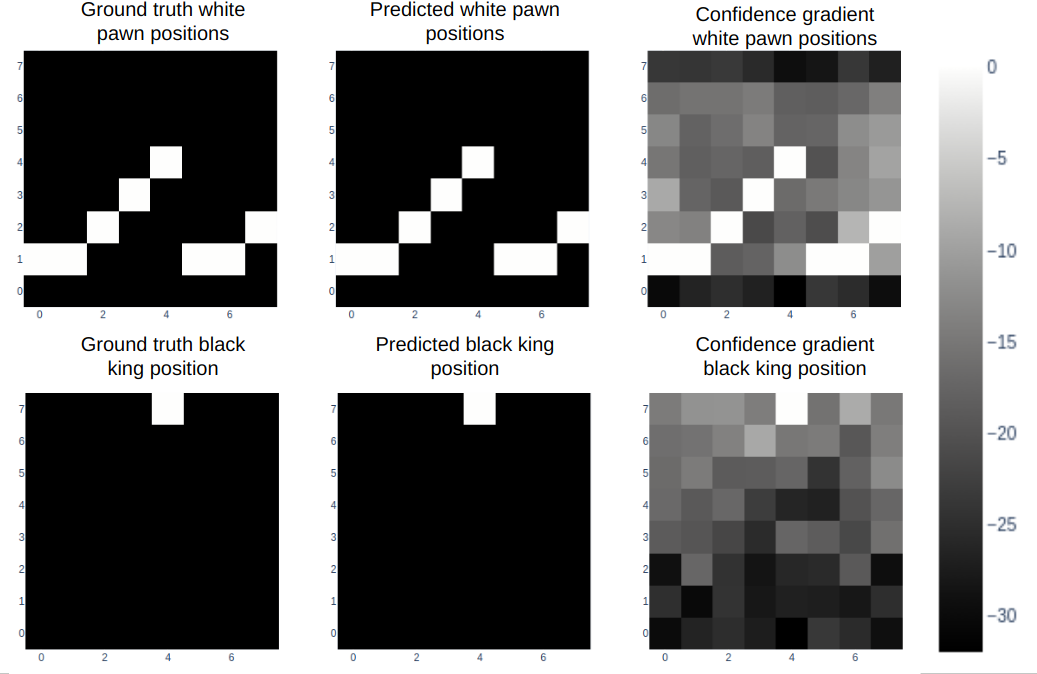
\includegraphics[width=0.85\textwidth]
        {figures/latent_space/probing_illustration.png}
    \caption{
        Probing analysis of a large language model trained to play chess
        \cite{karvonen2024emergentworldmodelslatent}.
    }
    \label{fig:probing_illustration}
\end{figure}

However, the fact that a concept can be decoded from \gls{lr} does not necessarily imply that the model actually uses this information to perform its task.
To assess whether \gls{lr} play a causal role in the model’s output, it is possible to perform interventions on them.
An intervention consists of modifying a \gls{lr} in a controlled manner by activating or deactivating a given concept, and then studying its impact on the model’s output.
If the resulting change in the model’s output is consistent with the applied perturbation, this suggests that the representation had a causal role.

To this end, the \gls{lr} is minimally modified such that the probe prediction for the target concept $c_j$ changes state, while the predictions associated with other concepts remain unchanged.
This goal can be formulated as an optimization problem over the \gls{lr} itself.
The optimization is performed directly on the \gls{lr}, using \gls{sgd}.
The solution to this problem is the optimal modified \gls{lr}, defined as:
\[
\latentRepresentation[l]^{*} =
\arg\min_{\latentRepresentation[l]'}
\underbrace{\gamma \, \mathcal{L}_{\text{flip}}\big(p_{\theta}^{l,j}(\latentRepresentation[l]'), c_j\big)}_{\text{flip target concept } c_j}
+
\underbrace{\lambda \sum_{k \neq j} \mathcal{L}_{\text{preserve}}\big(p_{\theta}^{l,k}(\latentRepresentation[l]'), c_k\big)}_{\text{preserve other concepts } c_{k \neq j}}
+
\underbrace{\beta \|\latentRepresentation[l]' - \latentRepresentation[l]\|_2^2}_{\text{minimality}}
\]
where:
\begin{itemize}
    \item $\latentRepresentation[l]$ is the original \gls{lr} of the input at layer $l$,
    \item $\latentRepresentation[l]'$ is the modified \gls{lr} being optimized,
    \item $\latentRepresentation[l]^{*}$ is the optimal modified \gls{lr},
    \item $\mathcal{L}_{\text{flip}}$: loss encouraging the prediction of the target concept $c_j$ to change state (i.e., flipping the predicted label),
    \item $\mathcal{L}_{\text{preserve}}$: loss enforcing invariance of all non-target concepts $c_k$ for $k \neq j$,
    \item $\|\latentRepresentation[l]' - \latentRepresentation[l]\|_2^2$: regularization term ensuring the modified \gls{lr} remains close to the original one,
    \item $\gamma, \lambda, \beta$: weighting coefficients controlling the trade-off between the intervention strength, the preservation of other concepts, and the minimality of the perturbation.
\end{itemize}

In the context of \gls{llm} studied previously, such interventions have been used to remove specific pieces from the model’s internal representation of the game state \cite{li2024emergentworldrepresentationsexploring, karvonen2024emergentworldmodelslatent}.
The main observation is that, in the vast majority of cases, the model behaves as if the piece had effectively disappeared.
The \gls{llm} continues to generate legal moves while correctly accounting for the absence of the removed piece.
This provides evidence for the causal role of these internal representations in the model’s behavior.

A main limitation of the probing approach is that the concepts under investigation must be predefined before any analysis can be performed.
This introduces a strong bias in what can be studied.
Moreover, annotating a dataset for each concept is extremely time-consuming and requires significant human effort.
Interventions in \gls{ls} are also difficult to interpret, as it is not always clear what constitutes a meaningful change in the network’s output under a given perturbation.

Moreover, probing methods provide a binary view of concepts, focusing on whether a given concept is present or absent in a \gls{lr}.
This binary perspective can be overly restrictive, as concepts may be represented in a more continuous manner.
To obtain a more detailed characterization of these representations, the next section turns to methods that describe a concept as a direction in \gls{ls} along which it varies continuously.